\documentclass[11pt,a4paper]{article}

\usepackage{graphicx,hyperref,amsmath,natbib,bm,url}
\usepackage[utf8]{inputenc} % include umlaute

% -------- Define new color ------------------------------
\usepackage{color}  
\definecolor{darkblue}{rgb}{0.15,0,0.37}
\definecolor{darkred}{rgb}{0.35,0,0.08}
\definecolor{mygrey}{rgb}{0.85,0.85,0.85} % make grey for the table
% --------------------------------------------------------

\hypersetup{
colorlinks=true,
hypertexnames=false,
colorlinks,		
linkcolor={black},
citecolor={black},
urlcolor={black},
%ocgcolorlinks, % this option changes the link color to black when the document is printed, for legibility in b/w 
pdfstartview={FitV},
unicode,
breaklinks=true
} 

\usepackage{microtype,todonotes}
\usepackage[australian]{babel} % change date to to European format
\usepackage[a4paper,text={16.5cm,25.2cm},centering]{geometry} % Change page size
\setlength{\parskip}{1.2ex} % show new paragraphs with a space between lines
\setlength{\parindent}{0em} % get rid of indentation for new paragraph
\clubpenalty = 10000 % prevent "orphans" 
\widowpenalty = 10000 % prevent "widows"

\hypersetup{pdfpagemode=UseNone} % un-comment this if you don't want to show bookmarks open when opening the pdf


\usepackage{mathpazo} % change font to something close to Palatino

%\usepackage[scaled=0.86]{berasans}
%\usepackage[scaled=1.03]{inconsolata}

%%%%%%%%% Uncomment the following two lines to use Helvetica as font %%%%%%%%%%%%%%%%%%%%%%%%%%%
%\renewcommand{\familydefault}{\sfdefault} % to use sans-serif font
%\usepackage{helvet} % use Helvetica font
%%%%%%%%%%%%%%%%%%%%%%%%%%%%%%%%%%%%%%%%%%%%%%%%%%%%%%%%%%%%%%%%%%%%%%%%%%%%%%%%%%%%%%%%%%%%%%%%%

% The following line defines a new environment that you can use to make text to Helvetica.
%\newenvironment{myhelvet}{\fontfamily{phv}\selectfont}{\par}


%\usepackage{bookman}
%\usepackage{tgpagella}
%\usepackage{mathpazo} % Uncomment to pick this font (I think it's Palatino)
%\usepackage{mathptmx} % Use font close to Times New Roman
%\usepackage[T1]{fontenc} \usepackage{fourier}

%%%%%%%%%% Garamond from Jens %%%%%%%%%%%%%%%%%%%%%%%%%%%%%%%%%%%%%%%%%%
%\usepackage[T1]{fontenc}
%\usepackage[osf]{ebgaramond}
%%%%%%%%%%%%%%%%%%%%%%%%%%%%%%%%%%%%%%%%%%%%%%%%%%%%%%%%%%%%%%%%%%%%%%%%%

%%%%% Define font %%%%%%
%\usepackage{kpfonts}
%\usepackage[T1]{fontenc}
%%%%%%%%%%%%%%%%%%%%%%%%


\usepackage{longtable, booktabs, tabularx} % for nice tables
\usepackage{caption,fixltx2e}  % for nice tables
\usepackage[flushleft]{threeparttable}  % for nice tables

\newcommand*{\myalign}[2]{\multicolumn{1}{#1}{#2}} % define new command so that we can change alignment by hand in rows

% -------- For use in the bibliography -------------------
\usepackage{multicol}
\usepackage{etoolbox}
\usepackage{relsize}
\setlength{\columnsep}{1cm} % change column separation for multi-columns
\patchcmd{\thebibliography}
  {\list}
  {\begin{multicols}{2}\smaller\list}
  {}
  {}
\appto{\endthebibliography}{\end{multicols}}
% --------------------------------------------------------


\usepackage[onehalfspacing]{setspace} % Line spacing

\usepackage[marginal]{footmisc} % footnotes not indented
\setlength{\footnotemargin}{0.2cm} % set margin for footnotes (so that the number doesn't stick out) 



\usepackage{pdflscape} % for landscape figures

\usepackage[capposition=top]{floatrow} % For notes below figure

% -------- Use the following two lines for making lines grey in tables -------------------
\usepackage{color, colortbl}
\usepackage{multirow}
% ----------------------------------------------------------------------------------------


% The following defines a footnote without a marker
\newcommand\blfootnote[1]{%
  \begingroup
  \renewcommand\thefootnote{}\footnote{#1}%
  \addtocounter{footnote}{-1}%
  \endgroup
}



%%%%%%%%%%%%%%%%%%%%%%%%%%%%%%%%%%%%%%%%%%%%%%%%%%%%%%%%%%%%%%%%%%%%%%%%%%%%%%%%%%%%%%%%%%%%
\begin{document}

\vspace*{0.5cm}

\thispagestyle{empty} % page number not shown on first page

\begin{center}
{\LARGE [Title]}\\[0.4cm]
 {\large name}\\[0.2cm]
  {\large \href{mailto:firstname.surname@uni-bonn.de}{\texttt{firstname.surname@uni-bonn.de}}}\\[0.2cm]
 {\large \today}\\
\end{center}

\blfootnote{\textsl{\textbullet \phantom{a} We wish to thank X1, X2 and X3.}}

\vspace*{-0.1cm}
\begin{center}
\begin{minipage}{0.9\textwidth}
\textbf{Abstract.} Lorem ipsum dolor sit amet, consectetur adipiscing elit. Vestibulum euismod ex porta, imperdiet leo a, laoreet urna. Morbi gravida dignissim vestibulum. Aenean mollis sit amet erat quis ultrices. Pellentesque tempus elementum finibus. Vivamus tincidunt sapien lectus, non sodales lorem ullamcorper in. Vestibulum ante ipsum primis in faucibus orci luctus et ultrices posuere cubilia Curae.
\end{minipage}
\end{center}


Mauris consequat sit amet nulla a eleifend. Phasellus tortor neque, efficitur ac dolor eget, ornare condimentum nulla. In nulla magna, pharetra at molestie et, pharetra nec massa. Nunc elementum diam lectus, eu commodo ligula venenatis et. Sed vitae aliquam quam. Mauris eu dui porttitor, sodales urna non, porta nisi. Proin non varius ipsum.

\cite{F1953} ultricies vel sapien sit amet dapibus. Curabitur maximus sagittis erat, vel interdum magna luctus et. Aliquam ligula enim, aliquet nec arcu vel, varius ultricies quam. In lobortis, diam in tempor suscipit, nibh nisi pellentesque velit, id aliquet libero odio sit amet arcu. Quisque diam lacus, molestie ac suscipit ac, ullamcorper non lacus. Nam sed ullamcorper eros. In feugiat ante sed elit placerat, sed ultricies odio mollis. Pellentesque sem arcu, auctor sit amet gravida vel, laoreet nec arcu. Mauris felis dolor, egestas ac odio ac, ultricies sodales urna. Nulla sit amet arcu nec elit rutrum tempus in sit amet odio. Vestibulum a posuere nisl.

\citep{E2011} in diam eget ligula imperdiet laoreet a ut justo. Vivamus ultrices rhoncus erat quis auctor. Etiam lorem neque, venenatis aliquam dolor ut, rhoncus fermentum magna. Morbi augue felis, auctor sit amet fermentum sit amet, ullamcorper id libero. Aenean lacinia dui malesuada condimentum rutrum. Vestibulum et egestas ante, ut dictum mi. Vivamus vel turpis aliquam, venenatis est sed, mollis tellus. Mauris in faucibus nisl, eget euismod ante. Mauris porttitor, nisl efficitur iaculis \cite{BBD2013}, est nunc dictum ipsum, quis venenatis nibh arcu ac lacus. Proin rhoncus felis non enim fermentum, eu tempor diam tempus. Nullam lacinia a ligula id pulvinar. Maecenas maximus urna bibendum magna tempor, feugiat ullamcorper eros tristique. Nunc consequat odio ut lorem fringilla, quis ultricies ex dictum. Ut fermentum nunc at libero varius fermentum. Sed a elit iaculis, molestie lectus lobortis, consequat risus.

Vestibulum id semper dolor. Mauris in commodo elit. Vivamus at molestie mi, eu ultrices eros. Nulla pulvinar erat arcu. Aliquam vitae tincidunt lacus. Phasellus convallis, eros eget semper gravida, mauris mi scelerisque magna, id interdum augue enim vel urna. Vivamus vehicula malesuada ultrices. Sed eu elit hendrerit, varius risus nec, cursus augue. Quisque efficitur urna et elit venenatis viverra. Suspendisse potenti. Fusce sit amet pharetra nibh, in porta ante.


\section{Analysis}
Suspendisse posuere lectus vitae libero tincidunt dignissim. Nulla in purus posuere, accumsan arcu ut, imperdiet odio. Nam rutrum fermentum sapien sit amet lacinia. Nunc et luctus erat. Lorem ipsum dolor sit amet, consectetur adipiscing elit. Aenean varius feugiat commodo. Donec turpis eros, iaculis iaculis molestie sed, convallis et diam. Cras malesuada non enim vitae dapibus. Fusce ultricies lectus sed dictum posuere. Sed pretium nunc eu orci gravida, vel varius arcu placerat. Nulla facilisi. Suspendisse mollis neque vel semper consequat. Proin laoreet ac ex eu condimentum.

Nulla luctus mauris id interdum accumsan. Praesent consequat eros quam, ac tempus risus mollis eget. In at sem vel dolor venenatis tempor sed quis felis. Vestibulum facilisis commodo felis id iaculis. Suspendisse potenti. Aliquam tellus dui, auctor eu nunc nec, ultrices fringilla justo. Nunc commodo lectus sed eros scelerisque auctor. Sed porta fringilla ultricies. Vivamus pharetra, libero ac eleifend pharetra, massa massa tincidunt sem, non tincidunt ipsum elit at neque. Integer mattis ligula ac dignissim euismod. Suspendisse bibendum elementum arcu, et facilisis ipsum elementum eu. Mauris at nisi in quam rutrum venenatis. Pellentesque in turpis vel tellus pellentesque malesuada at eget arcu. Maecenas vitae nibh ipsum.


\begin{figure}
\caption{Cyclically adjusted monthly price earnings ratio}
	\centering
	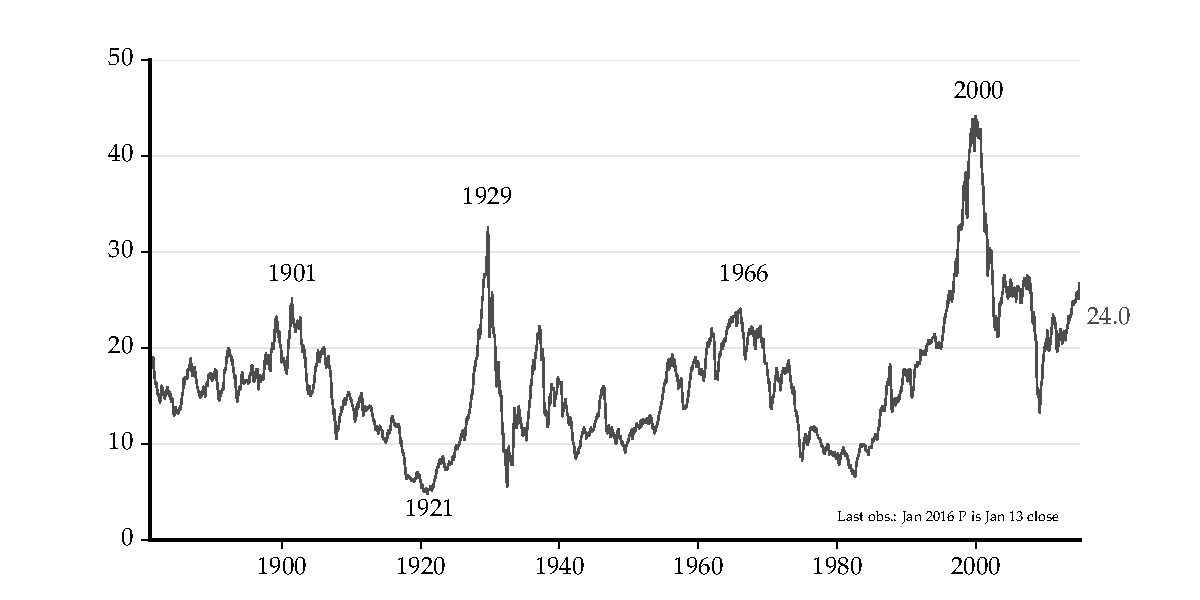
\includegraphics[trim=0cm 0cm 0cm 0cm, clip=true, totalheight=0.3\textheight]{figures/pe_ratio}
	\floatfoot{
	\begin{minipage}{0.65\textwidth}
	\textit{Source:} Robert J. Shiller (2015), {\href{www.irrationalexuberance.com}{\texttt{Irrational Exuberance}}}
	\end{minipage}
	}
	\label{fig:shiller_pe}
\end{figure}


Aenean ligula tortor, vestibulum non justo vitae, bibendum rutrum neque. Maecenas lobortis sit amet tellus eu varius. Nunc laoreet velit et velit maximus scelerisque. Aliquam erat volutpat. Aliquam placerat congue ultricies. Nam id mi fermentum, sagittis ligula eu, mollis orci. Vivamus turpis arcu, vehicula tincidunt bibendum condimentum, tempus in massa. Class aptent taciti sociosqu ad litora torquent per conubia nostra, per inceptos himenaeos. Suspendisse vitae elementum lorem. Aliquam sodales augue magna, vitae porta risus finibus quis. Mauris vel aliquam mauris, a fermentum tortor. Nulla nec faucibus mi. Nullam venenatis, nibh dictum placerat vehicula, est elit vehicula velit, non dignissim magna nisi sit amet libero. Aliquam eu eleifend ipsum. Cras at arcu sit amet massa pharetra posuere vitae quis magna.



%%%%%%%%%%%Bibliography%%%%%%%%%%%
\vspace*{0.5cm}
\setstretch{1} % Set line spacing to 1 for the bibliography.
\begin{thebibliography}{9}
	\bibitem[Baker et al.(2013)]{BBD2013} \textbf{Baker, Scott R., Nicholas Bloom and Steven J. Davis} (2013). ``Measuring Economic Policy Uncertainty." \textit{Chicago Booth research paper}, 13-02.	

	\bibitem[Eichengreen(2011)]{E2011} \textbf{Eichengreen, Barry} (2011). \textit{Exorbitant Privilege: The Rise and Fall of the Dollar and the Future of the International Monetary System}, Oxford University Press.

	\bibitem[Friedman(1953)]{F1953} \textbf{Friedman, Milton} (1953). ``The Case for Flexible Exchange Rates". \textit{Essays in Positive Economics}, University of Chicago Press.

	\bibitem[International Monetary Fund(2014)]{IMF2014} \textbf{International Monetary Fund} (2014). \textit{Annual Report on Exchange Arrangements and Exchange Restrictions}.

\end{thebibliography}



%%%%%%%%%%%%%%%%%%%%%%%%%%%%%%%%%%%%%%%%%%%%%%
\end{document}
